\documentclass[journal, draftcls]{IEEEtran}
% Add the compsoc option for Computer Society conferences.
%
% If IEEEtran.cls has not been installed into the LaTeX system files,
% manually specify the path to it like:
% \documentclass[conference]{../sty/IEEEtran}


\usepackage[usenames]{color}
\usepackage{graphicx}
\usepackage{multirow}
\usepackage{caption}
\usepackage{subcaption}
\usepackage{url} 
\usepackage{enumerate}
\usepackage{flushend}

\usepackage{caption}
\usepackage{subcaption}
% DOCUMENT

\usepackage{draftwatermark}



\begin{document}
%
% paper title
\title{Statement of Purpose}
\author{
\IEEEauthorblockN{Ryan A. Rodriguez}
\IEEEauthorblockA{\\Undergraduate, Department of Electrical Engineering\\UC Santa Cruz, Santa Cruz, CA 95064\\
Email: ryarodri@ucsc.edu, URL: http://www.empireryan.com}
}
\maketitle
\section{Introduction}

Getting a graduate education is essential for my development as a competent engineer, researcher, and entrepreneur in the fields of robotics, cyber-physical and embedded systems. The countless hours of study, all-nighters in the lab, triumphs, and the far more numerous failures in my undergraduate career have shown me just how much I still have to learn, and reaffirmed my commitment to a lifetime of scholarship and innovation. As I've expanded my skill-set, I have consistently felt the need to push my  boundaries and reach beyond what I think I can accomplish. The logical next step in my progression is to pursue the PhD in Electrical Engineering at \textit{{school name here}} to deepen my technical knowledge in the field, to hone my ability to conduct world-class research and to push the limits of my profession. 

\section{Background}
\subsection{Project 1}
My first real encounter with a problem demanding exhaustive research was during the spring of my junior year at UC Santa Cruz. I had enrolled in my first graduate course in microelectromechanical systems taught by Dr. Joel Kubby, and the final project was to design a continuous face-sheet deformable mirror to be used for adaptive optics. The design requirements called for micrometer scale actuators that had to be powerful enough to deform the gold and poly-silicon mirror surface, but also needed to maintain a linear operation at strokes past two-thirds of the initial electrode gap. The region beyond this point is typically characterized by unstable performance and a pull-in phenomena due to the linear restoring force being overwhelmed by the non-linear coulomb force. A simple fix is to simple increase one initial gap between electrodes to achieve the desire linear region; however, this is not possible in the multi-user process that we were constrained by. After some days of sifting through MEMS journals I stumbled upon a paper by Edward Chan and Robert Dutton that described the use of series capacitance to allow for extended stroke in MEMS actuators. This innovative use of capacitance came from the realization that  the actuator itself is a capacitor, and that we can simulate a larger gap by increasing the capacitance seen by the control mechanisms. While the electromagnetic theory was ingenious, their folded spring design saw astable, positive feedback from asymmetries introduced in the manufacturing process. Though the authors deemed this problem a fundamental limitation of the technology, I was convinced I had the solution to the instability problem; by using fixed-guided springs in an 'X' pattern my design would have a stiffer response than Chan and Dutton's folded springs while also forming a negative mechanical feedback loop. If any one corner of the X-beam design begins to pull in faster than the others, the non-linear nature of the springs causes the restoring force to increase rapidly. This allows for the actuator to maintain equilibrium throughout an extended range of travel. 
I rounded out my design by folding the requisite capacitors into the trapezoidal spaces left by the X-beam actuator. This dense layout eliminated the effect of empty space in lower silicon layers from producing unwanted topography on the mirrored surface above. Ultimately, the research pushed me to develop electrical and mathematical models to optimize my design, and to become adept at using finite element analysis to test my hypothesis. As an undergraduate with a chip on my shoulder in a class full of graduate students not only did my design achieve the largest stable stroke, but I supported my results with an overwhelming amount of evidence and research.  

\subsection{Project 2}
That Summer I had been offered a National Science Foundation grant to work with the Team for Research in Ubiquitous Secure Technology at UC Berkeley for an undergraduate research experience. Out of a select group, I was chosen to work on the Tigres project with the Advanced Computing for Science division at Lawrence Berkeley National Laboratory under Dr. Lavanya Ramakrishnan. Tigres is a Python API born of the realization that the vast majority of scientific workflows can be composed from a small set of computational patterns. Tigres was designed to streamline the process of composing and executing data intensive scientific workflows on a wide array of high performance commuting resources. Although it has been found that scientists prefer to hand code their workflows, almost all modern workflow managers turn to a visual interface. My research during that summer focused on the feasibility and design of a versatile interface that would allow a scientists' hard-coded workflows to be visualized instantly, and for changes in a visual editor to generate the code needed to execute a given workflow. A third aspect of the interface was a command line interface that could generate complex workflows with a very compact instruction set. This active console and visual editor offered scientists the flexibility of code while allowing for valuable visual feedback and time-saving code generation tools. 

\subsection{Project 3}
 The following Fall quarter I enrolled in Dr. Gabriel Elkaim's Introduction to Mechatronics course. The class is notorious for being among the most challenging - if not the most challenging - in the department of engineering at UC Santa Cruz, so naturally I was drawn to its cult status. The course crams Stanford's three quarter long mechatronics design experience into a single quarter where teams of 3-5 students build a fully autonomous rover capable of completing an obstacle course while firing ping-pong balls at an opposing robot. My experience was nothing short of transformative because instead of just learning theory, I was responsible for building and coding everything we had covered in class by hand. By the end, I had a firm grasp on motor and speed control, analog and digital filter implementations, rapid prototyping and the fundamentals of robust, autonomous, embedded system design. My team's finished automaton used a pair of selective IR beacon detector circuits to target enemy robots with its turret, and a set of stepper motors with a software pedometer to estimate its position.  

\subsection{Project 4}
 I spent the following two quarters performing independent research on embedded systems and decentralized workflow execution using Tigres, and taking coursework at the prestigious University of Ghana in West Africa. My research with Tigres  focused on the feasibility and implementation of techniques used in MapReduce implementations to data intensive science on exascale computers. This philosophy demands the implementation of decentralized workflow managers in a departure from today's highly centralized systems. During this time I not only began to conceptualize how Tigres could be used to design and execute cyber-physical systems, but also to take a step back from the purely technical nature of engineering to examine the ethics of what it is we do. 
 
 In Ghana I got to see the troubling societal and environmental costs of our technological rush and the information gap between the first and third world. It was no longer an option for me to stream lectures that I needed to review, download books or conduct research online with a first world internet connection. It was truly sobering seeing students and scholars with no less drive than me having to conduct their academic careers on internet connections that were typically slower than the 56k of my youth. Until I saw them for myself, I had never truly considered my role in the creation of sprawling, toxic, electronic trash heaps in developing countries. Words cannot describe how I felt as I watched people working in carcinogenic plumes of smoke to sort the scrap metal out of our discarded electronics. I decided to become an engineer to do the most good, to advance humanity and push the bounds of what we know. My time at UG has shown me that this has not been the net effect of the past generation of engineering breakthroughs; rather, we've seen a large percentage of the globe left behind. 

\section{Objectives}
Peter Kinget
Mingoo Seok

The PhD in Electrical Engineering with a focus in \textit{{put research focus here}} at \textit{{put school here}} is the right fit for me because it will further my capability to do research while also preparing me to become a future business leader capable of effecting change globally. 

\begin{IEEEbiography}
[{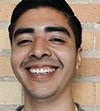
\includegraphics[width=1in,height=1.25in,clip,keepaspectratio]{./RodriguezR.jpg}}]{Ryan Rodriguez} was born in 1989 and completed his elementary and secondary education in the East Bay Area. He is a graduate of the USAF's ground radio and satellite communication school at Keesler AFB in Biloxi, MS where he also earned an FBI level 'Secret' security clearance. Ryan is currently completing the final year of his BS in Electrical Engineering at UC Santa Cruz, and finishing his senior design and research cycle. Ryan is interested in MEMS, mechatronics, embedded and cyber-physical systems, the economics of information, entrepreneurship and law. 
\end{IEEEbiography}

\end{document}
